% Made up for the tikra gallery: shader=interp blends the colors between the points of the mesh.
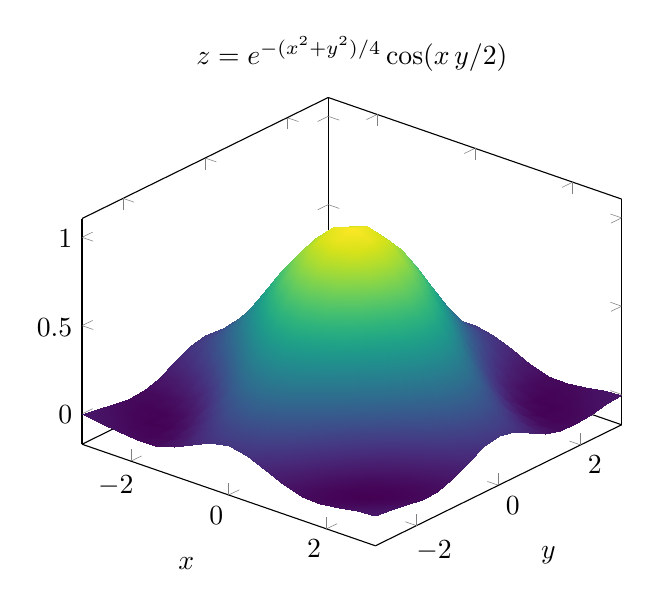
\begin{tikzpicture}
\begin{axis}[view={40}{35}, colormap/viridis, xlabel=$x$, ylabel=$y$,
    title={$z = e^{-(x^2+y^2)/4}\cos(x\,y/2)$}]
  \addplot3[surf, shader=interp, domain=-3:3, y domain=-3:3, samples=17]
    {exp(-(x^2+y^2)/4)*cos(deg(x*y/2))};
\end{axis}
\end{tikzpicture}
